\documentclass[12pt]{beamer}
\usetheme{Singapore}
\usepackage{mathpazo}
\renewcommand{\rmdefault}{ppl}
\setbeamerfont{title}{family=\rmfamily}
\setbeamerfont{frametitle}{family=\rmfamily}
\usepackage[utf8]{inputenc}
\usefonttheme{professionalfonts} 
\usepackage{amsmath}
\usepackage{amsfonts}
\usepackage{amssymb}
\usepackage{xcolor}
\usepackage{tikz}
\usetikzlibrary{positioning,fit}

\author{Lai Hao Ran \\ \footnotesize\texttt{hrlai.ecology@gmail.com}}
\title{Basic introduction to\\Bayesian inference}
\date{} 
%\setbeamercovered{transparent} 
\setbeamertemplate{navigation symbols}{} 

\titlegraphic{%
	\centering
	
\includegraphics[height=0.15\textheight]{fig/Marsden-logo-RGB-150.jpg}~%
	\hspace{1cm}
	
\includegraphics[height=0.15\textheight]{fig/University_of_Canterbury_logo.png}~%
	\hspace{1cm}
	
\includegraphics[height=0.15\textheight]{fig/searpp.png}
} 

\newcommand\blfootnote[1]{%
  \begingroup
  \renewcommand\thefootnote{}\footnote{#1}%
  \addtocounter{footnote}{-1}%
  \endgroup
}

\begin{document}

\begin{frame}
\titlepage
\end{frame}

\begin{frame}{Today's plan}
Part 1:
\begin{itemize}
\item Three ways to write (and read) a model
\item (Generalised) linear regression
\end{itemize}

Part 2:
\begin{itemize}
\item How to make a model go?
\item Interpreting outputs
\end{itemize}
\vfill
We will not explicitly cover:
\begin{itemize}
\item Bayes theorem 
\item Priors
\end{itemize}
\end{frame}

\begin{frame}{Why?}
How Bayes reshaped my thinking (for better or worse):
\begin{enumerate}
\item I understand GLMs better
\item I stop worrying about $p$-values and start to be comfortable with uncertainties
\item I begin to see my model as modular; when it fails to converge, I understand which part was the culprit
\item It is slower, so you think harder about your model
\item I understand the meaning of each parameter, including the variance term
\item I can map my parameters to my questions
\item My models become \textbf{more purposeful}
\end{enumerate}
\end{frame}

\begin{frame}{Three ways to write (and read) a model}
\begin{enumerate}
\item Graphical
\item Code
\item Maths
\end{enumerate}
\vfill
Pair up
\end{frame}

\begin{frame}{The graphical way}
The effect of temperature on diversity.

\only<1>{
\begin{center}
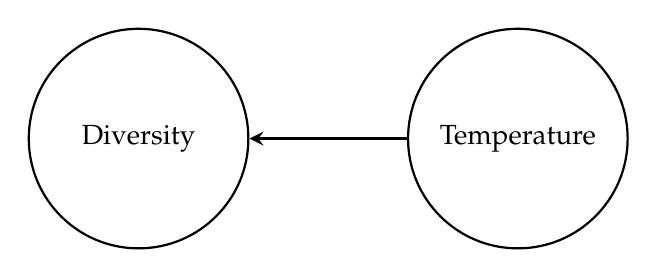
\begin{tikzpicture}[
roundnode/.style={circle, draw, thick, text width=2.5cm, align=center},
]
%Nodes
\node[roundnode] (y) {Diversity};
\node[roundnode] (x) [right=2cm of y] {Temperature};
%Lines
\draw[-stealth, very thick] (x) -- (y);
\end{tikzpicture}
\end{center}
}

\only<2>{
\begin{center}
\begin{tikzpicture}
\draw[-, thick] (0,0) -- node[anchor=north]{Temperature} (5,0);
\draw[-, thick] (0,0) -- node[anchor=south, rotate=90]{Diversity} (0,5);
\end{tikzpicture}
\end{center}
}

\end{frame}

\begin{frame}{The code way}
\begin{center}
\texttt{lm(Y $\sim$ 1 + X)}
\end{center}
\end{frame}

\begin{frame}{The maths way}
$$ Y = a + bX + \epsilon $$
\begin{align*}
Y &\sim \text{Normal}(\mu, \sigma_\epsilon) \\
\mu &= a + bX
\end{align*}
\end{frame}

\begin{frame}{Back to the graphical way}
\begin{center}
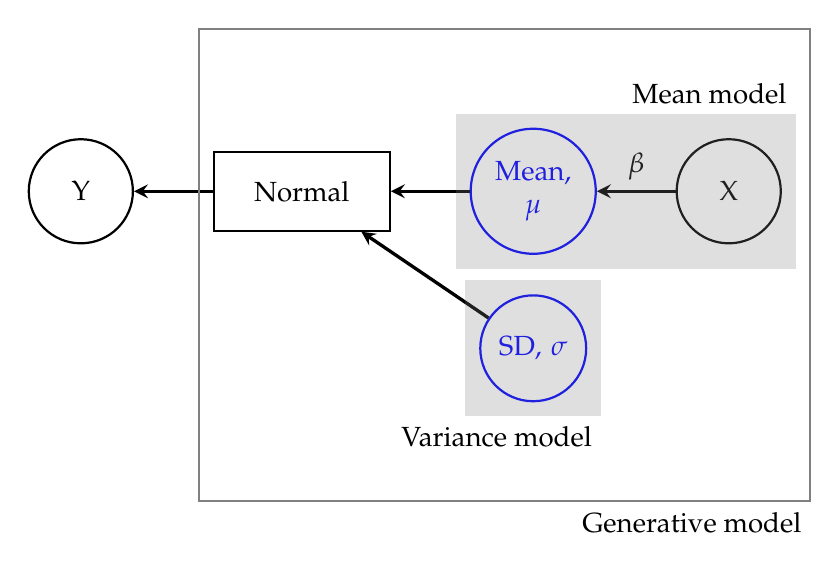
\begin{tikzpicture}[
roundnode/.style={circle, draw, thick, text width=1cm, align=center},
rectnode/.style={rectangle, draw, thick, text width=1cm, align=center},
]
%Nodes
\uncover<1->{ \node[roundnode] (y) {Y}; }
\uncover<3->{ \node[rectnode] (distr) [right=1cm of y, text width=2cm, minimum height=1cm] {Normal}; }
\uncover<2->{ \node[roundnode, blue] (mu) [right=1cm of distr] {Mean, $\mu$}; }
\uncover<1->{ \node[roundnode] (x) [right=1cm of mu] {X}; }
\uncover<4->{ \node[roundnode, blue] (phi) [below=0.5cm of mu] {SD, $\sigma$}; }
%Lines
\uncover<2->{ \draw[-stealth, very thick] (x) -- node[anchor=south]{$\beta$} (mu); }
\uncover<3->{ \draw[-stealth, very thick] (mu) -- (distr); }
\uncover<4->{ \draw[-stealth, very thick] (phi) -- (distr); }
\uncover<5->{ \draw[-stealth, very thick] (distr) -- (y); }
% boxes
\uncover<6->{ 
\node[inner sep=5pt,fill=gray,nearly transparent,fit=(mu) (x)] (meanmod) {};
\node[above left] at (meanmod.north east) {Mean model};
}
\uncover<7->{ 
\node[inner sep=5pt,fill=gray,nearly transparent,fit=(phi)] (varmod) {};
\node[below left] at (varmod.south east) {Variance model};
}
\uncover<8->{ 
\node[inner sep=5pt,draw,gray,thick,minimum height=6cm,fit=(distr) (varmod) (x) (meanmod)] (genmod) {};
\node[below left] at (genmod.south east) {Generative model};
}
\end{tikzpicture} 
\end{center}
\end{frame}

\begin{frame}{What happens if the response is not Normal?}
\begin{align*}
Y &\sim \textcolor{blue}{\text{Distribution}}(\mu,~\phi) \\
\textcolor{blue}{\text{Link-function}}(\mu) &= a + bX
\end{align*}
\end{frame}

\begin{frame}{When should I stop?}
\begin{itemize}
\item Bayesian inference is flexible, therefore it is a rabbit hole
\item When you spend too much time building ever more complex Bayesian models, it is probably a good time simplify your questions instead
\item At which point you may find that you don't need Bayes anyways
\end{itemize}
\end{frame}

\begin{frame}
I still use frequentist approach, and everytime I return to it, I realise how much more I appreciate frequentist because of what I have learnt from Bayesian inference.
\end{frame}

\end{document}